\usepackage{epstopdf}

\begin{document}

\section{Methods}\label{sec:Methods}
In order to create histograms showing when the warmest and coldest days typically occurred from $1722$ up to $2013$ in Uppsala, two
arrays respectively storing the hottest and coldest day for each year are needed. A code was written in order to read the data of
the SMHI recorded from Uppsala and then produce two output files:
\begin{itemize}
\item one cointaining a list of the years with the corresponding hottest and coldest days; 
\item one containing most of the recorded temperatures (some of them were excluded as explained below) with the corresponding day 
(from 1 to 366) and year.
\end{itemize}

Since not all the data contained in the file from the SMHI were recorded from the same place, all the readings from a region other
than Uppsala were ignored. In the first output file the code returns $0$  for the years in which no temperature was measured in
Uppsala (and also for the corresponding hottest and coldest days). In the second output file a line of "$0$" is present for each 
temperature not recorded in the region of interest.

The data from the Uppsala.dat file are read into a two dimensional array.The functions Function{\_}max and Function{\_}min are used
inside a loop over the first column of the array (containing all the years associated to the temperatures recorded in the 
SMHI file) in order to find the hottest temperature and the coldest temperature of each year with the associated days. The maximization
and minimization are achieved by comparing each temperature with the one stored in the following line, so that the higher/lower temperature between 
the two is written over the one previously stored in the variable Tmax{\_}temporary or Tmin{\_}temporary.The two functions store temperature and day in an array and return the pointer to the array. The function NumberoutofDate
is used in the two function mentioned above and, by taking the 2 dimensional array and the line of the hottest/coldest temperature
as input, it returns a number between 1 and 366 corresponding to the day in which that specific temperature has been recorded. 
The loop cycle in which the functions mentioned above are called produces an array containing a list of the years, and 2 arrays 
containing the hottest and coldest days respectively. These three arrays are printed in the first output file of the code.
The arrays needed to produce the second output file are generated in the second loop of the code.

A second code was then written in order to read the files produced by the first code and store the data of each column in a different 
array, but excluding the lines containing $0$ in the first column. An array is produced for each column of the two files and the 
arrays so obtained are exploited for producing graphs and histograms with ROOT.
Two overlaying histograms are produced, by calling the class T1H: one for the distribution of the hottest days and one showing the distribution of the 
coldest days. The histogram for the hottest days is fitted with a gaussan function and the mean of the distribution is returned with its 
uncertainty in order to predict when the hottest day is more likely to occur. The second histogram is fitted with 
two gaussian functions since the hottest days mainly occur both at the end of the year and at the beginning. The years are
plotted either against the corresponding hottest days and coldest days in two separate graphs, by calling the class TGraph. 

The 2DGraph class in ROOT is used to obtain a tridimensional graph showing how the temperatures in Uppsala changed over the days of 
the years from 1722 to 2013.


\section{Results}\label{sec:Results}

The overlaying histograms showing the distribution of the hottest and the coldest days are shown in figure \ref{fig:HotColdHist}.
The mean obtained for the distribution of the hottest days is $193 \pm 2$. The graphs showing how the hottest days and coldest days 
changed over the years are shown in Figures  \ref{fig:HotGraph} and \ref{fig:ColdGraph}. 


\begin{figure}[h]
\begin{center}
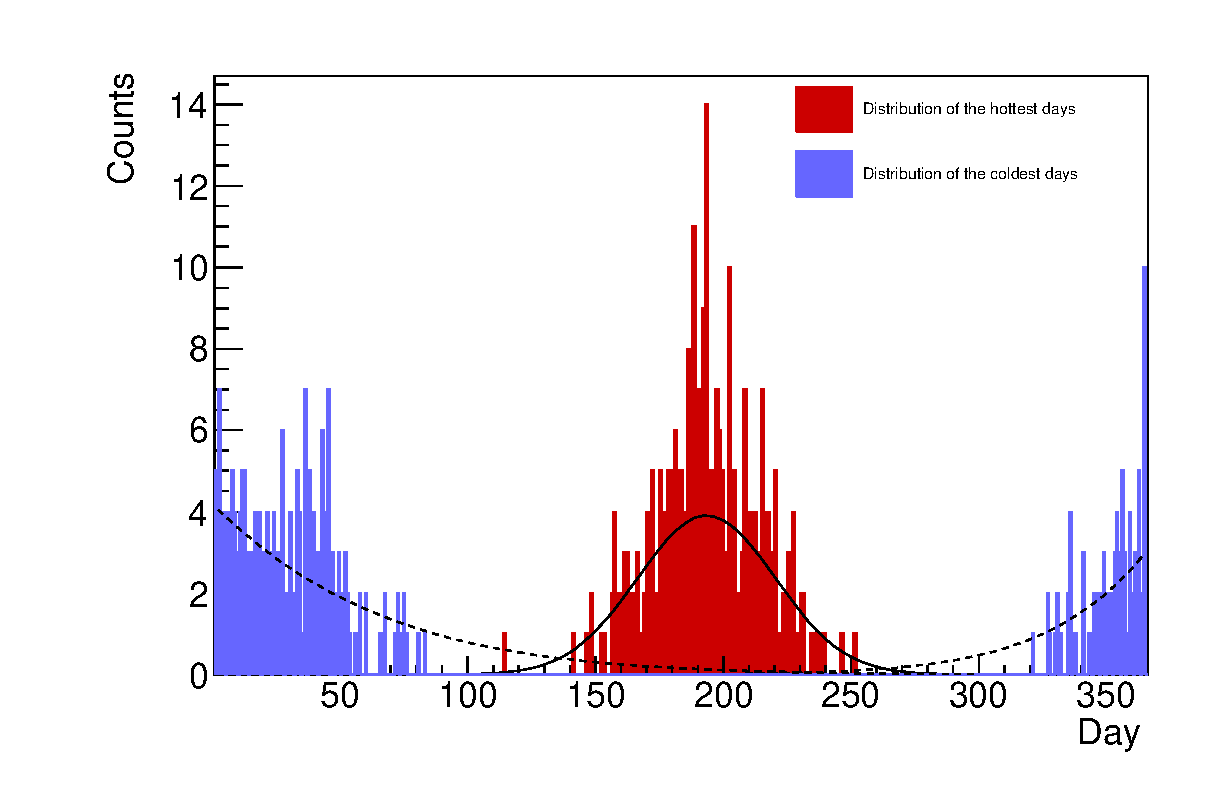
\includegraphics[width=12cm]{HottestColdest.eps}
\caption{Histogran showing how often each day of the year was the warmest or coldest from 1722 to 2013. Lines 
show Gaussian fits of the two distributions.}
\label{fig:HotColdHist}
\end{center}
\end{figure}

\begin{figure}[h]
\begin{center}
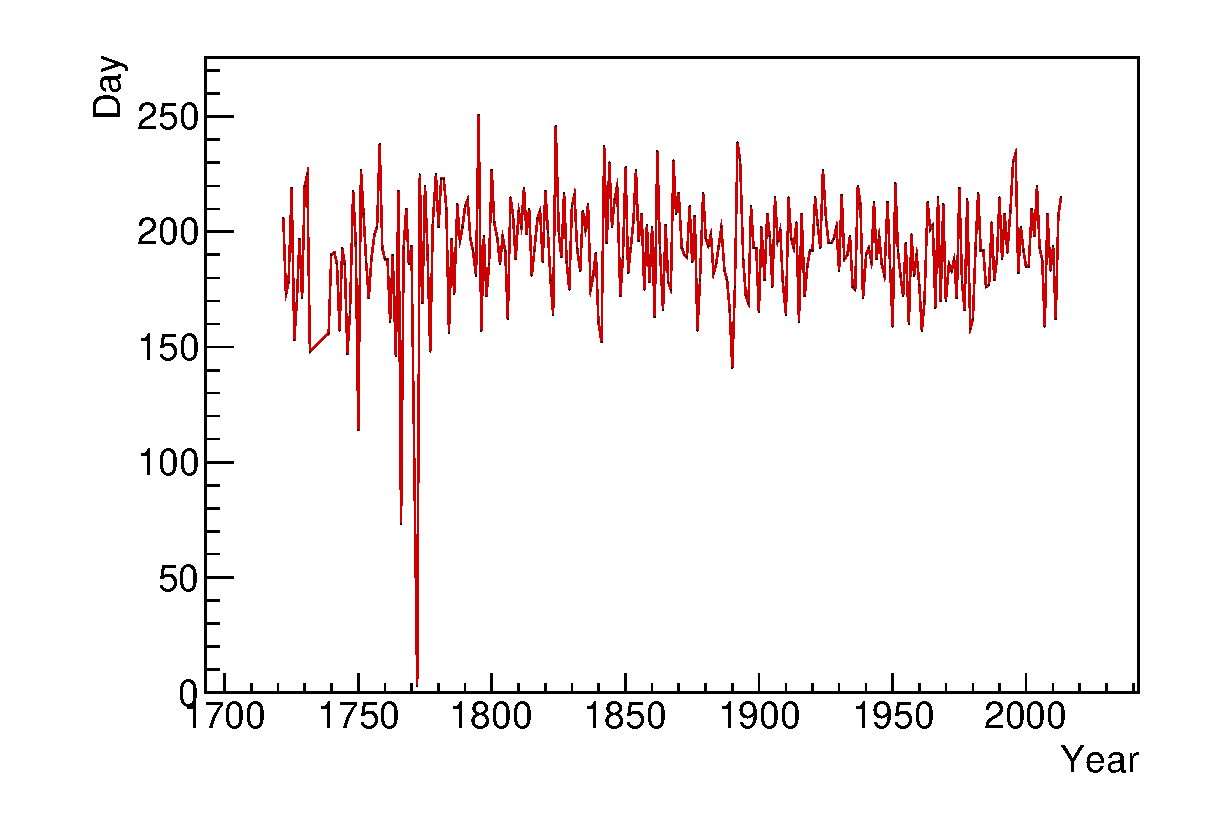
\includegraphics[width=12cm]{graph1DHot.eps}
\caption{Graph showing how the temperatures in Uppsala changed over the days of the years from 1722 to 2013..}
\label{fig:HotGraph}
\end{center}
\end{figure}

\begin{figure}[h]
\begin{center}
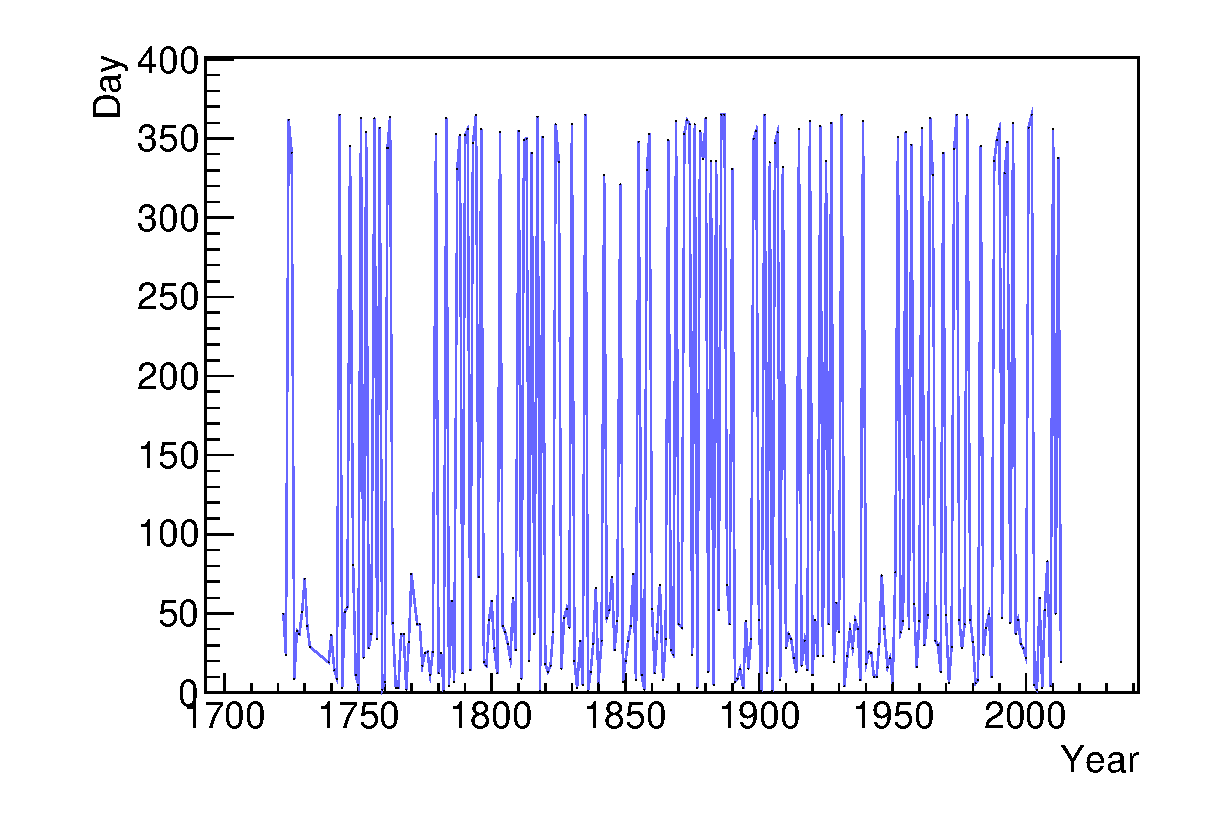
\includegraphics[width=12cm]{graph1DCold.eps}
\caption{View from the top of the Graph in figure \ref{fig:3D}.}
\label{fig:ColdGraph}
\end{center}
\end{figure}

\begin{figure}[h]
\begin{center}
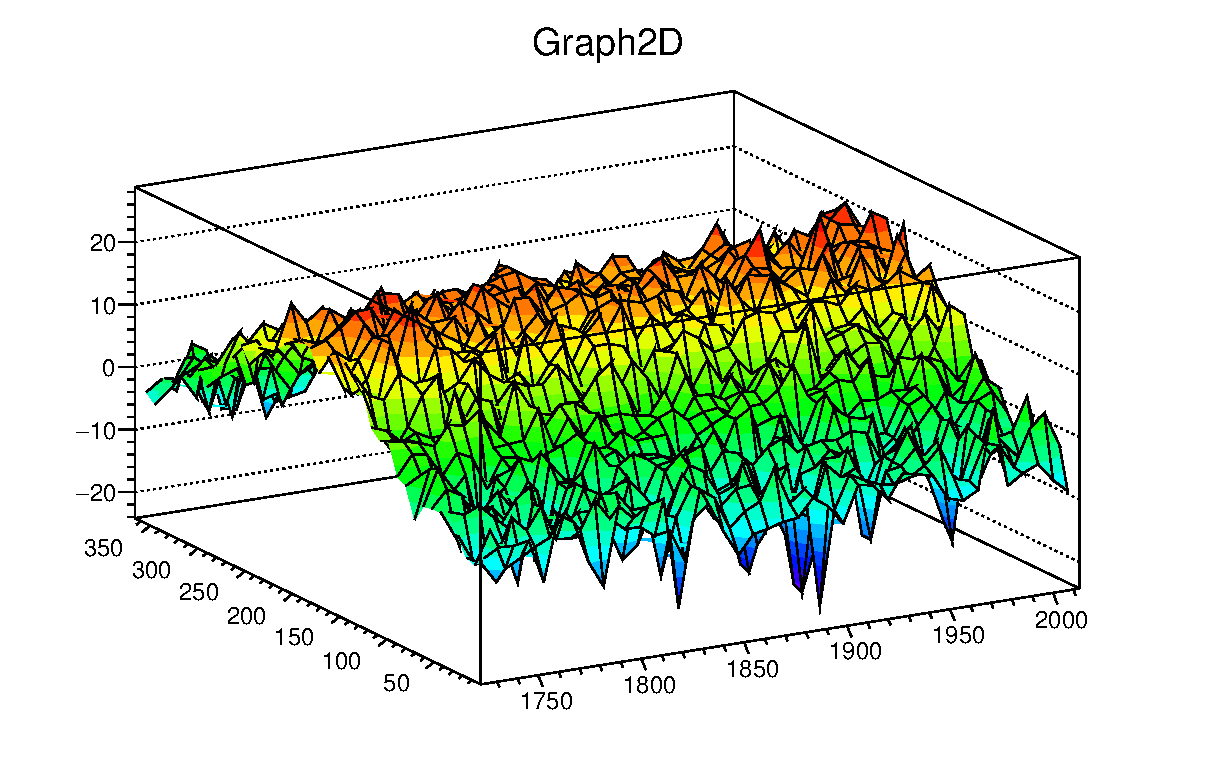
\includegraphics[width=12cm]{2Dgraph1.eps}
\caption{Graph showing the coldest.}
\label{fig:3D}
\end{center}
\end{figure}

\begin{figure}[h]
\begin{center}
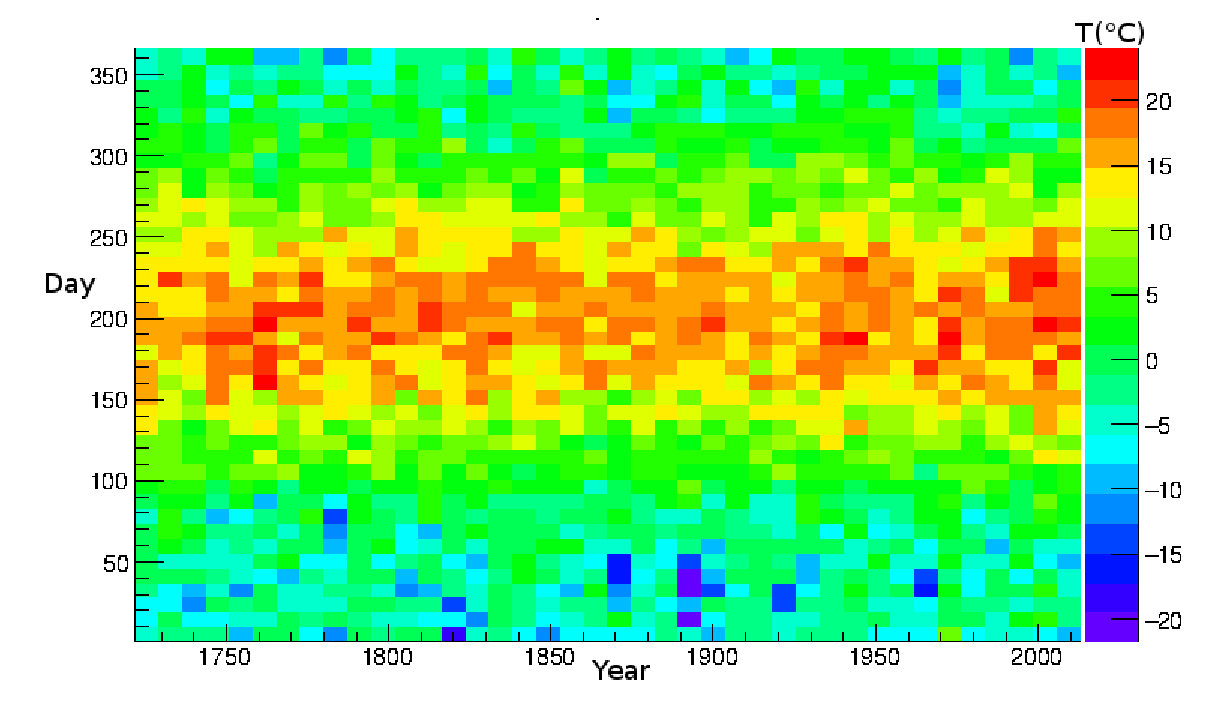
\includegraphics[width=12cm]{2Dgraphint.eps}
\caption{Graph showing the coldest day for each year.}
\label{fig:top3D}
\end{center}
\end{figure}

\section{Discussion}\label{sec:Discussion}
Figure \ref{fig:HotColdHist} shows that the hottest temperature in Uppsala is most likely to be registered around day $193$

%\begin{thebibliography}{99}

%\end{thebibliography}

 
 \end{document}
